
\subsection{Аннотация:}
В ходе данной работы в целях ознакомления применены различные методы получения и анализа поляризованного света. Рассмотрены явления линейной и эллиптической поляризации света, а также интерференции поляризованных лучей. Качественно определены разрешённые направления поляроидов, характер поляризации света при отражении и преломлении, главные направления двоякопреломляющих пластин, положения <<медленной>> и <<быстрой>> осей и направление вращения вектора напряжённости электрического поля при эллиптической поляризациии. 

\subsection{Оборудование:} 
Оптическая скамья с осветителем; зелёный светофильтр; два поляроида; чёрное зеркало; полированная эбонитовая пластинка; стопа стеклянных пластинок; слюдяные пластинки различной толщины; пластинки в 1/4 и 1/2 длины волны; пластинка в одну длину волны для зелёного света (пластинка чувствительного оттенка).

%-------Teor---------------------------

\par
\subsection{Теоретические сведения:} 

\subsubsection{Определение направления разрешённой плоскости колебаний поляроида}
	
Определить направление разрешённых колебаний поляроида проще всего с помощью чёрного зеркала. При падении света на отражающую поверхность под углом Брюстера свет в отражённом луче почти полностью поляризован, а вектор $\mathbf{E}$ параллелен отражающей поверхности. Луч света, прошедший поляроид и отразившийся от чёрного зеркала, имеет минимальную интенсивность при выполнении двух условий: во-первых, свет падает на отражающую поверхность под углом Брюстера и, во-вторых,
в падающем пучке вектор E лежит в плоскости падения.

Вращая поляроид вокруг направления луча и чёрное зеркало вокруг оси, перпендикулярной лучу, методом последовательных приближений можно добиться минимальной яркости луча, отражённого от зеркала, и таким образом определить разрешённое направление поляроида. Зная угол поворота зеркала (угол Брюстера), можно определить коэффициент преломления материала, из которого изготовлено
зеркало. Из определения угла Брюстера следует
\begin{equation} \label{BrewstersAngle}
    n = \tg{\varphi_\text{Б}}.
\end{equation}

\subsubsection{Получение эллиптически поляризованного света}

Эллиптически поляризованный свет можно получить из линейно поляризованного с
помощью двоякопреломляющих кристаллических пластинок.

Двоякопреломляющая пластинка имеет два взаимно перпендикулярных главных направления, совпадающих с осями эллипсоида диэлектрической проницаемости. Волны, поляризованные вдоль главных направлений, распространяются в пластинке с разными скоростями, не изменяя характера своей поляризации. Эти волны называются главными. Мы будем обозначать показатели преломления для главных волн через $ n_x $ и $ n_y $, где $ x $ и $ y $ --- главные направления кристаллической пластинки (рис. \ref{pic_1}).
\begin{figure}[!hb]
	\centering
	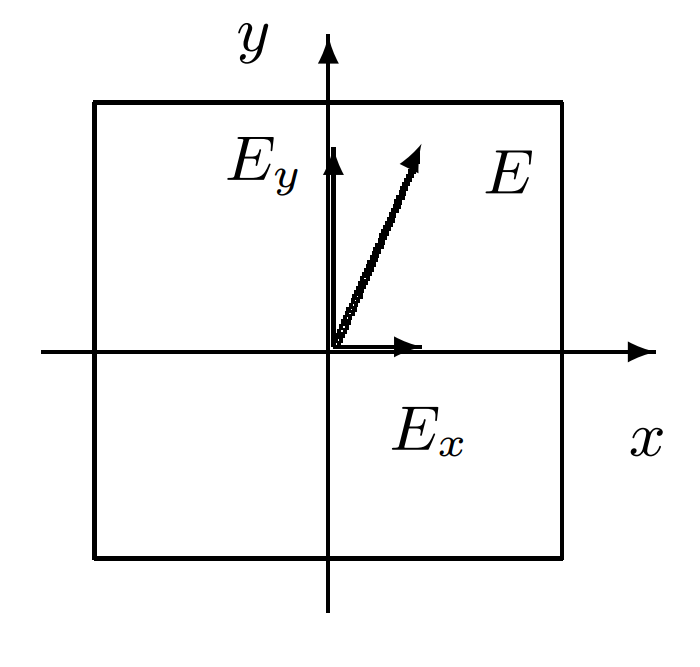
\includegraphics[width=0.3\linewidth]{pics/pic_1.png}
	\caption{{ Разложение линейно поляризованного света по главным направлениям двоякопреломляющей пластинки}}
	\label{pic_1}
\end{figure}

Пусть на пластинку падает линейно поляризованная волна, электрический вектор которой ориентирован под некоторым углом $\alpha$ к оси
$x$. Разложим вектор $\mathbf{E}$ на составляющие $E_x$ и $E_y$. На входе пластинки $E_x$ и $E_y$ находятся в фазе. На выходе из-за разности скоростей между ними появляется разность хода $d(n_x - n_y)$, при этом сдвиг фаз определяется соотношением
\begin{equation}\label{PathDiff}
\Delta \varphi =  \dfrac{2\pi}{m} = k d(n_x - n_y)
\end{equation}

Как уже отмечалось, при сложении двух взаимно перпендикулярных колебаний, обладающих некоторым сдвигом фаз, образуется колебание, поляризованное по эллипсу.

\begin{figure}[!hb]
	\centering
	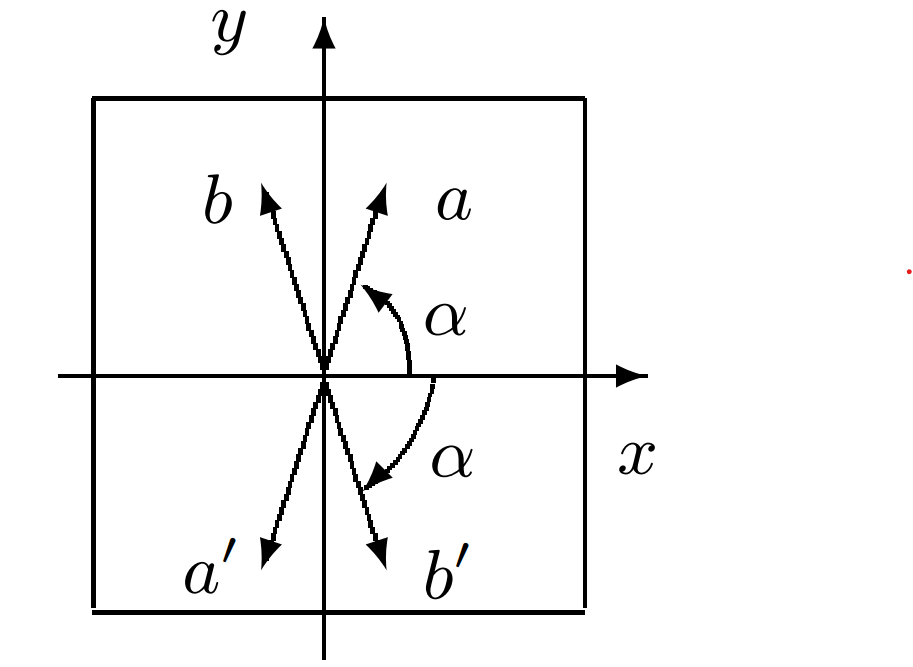
\includegraphics[width=0.35\linewidth]{pics/pic_2.png}
	\caption{{Поворот направления колебаний с помощью пластинки в $\lambda/2$}}
	\label{pic_2}
\end{figure}

Рассмотрим практически важные частные случаи.

\begin{enumerate}
 		
\item Пластинка даёт сдвиг фаз $ 2\pi $ (пластинка в длину волны $ \lambda $). В результате сложения волн на выходе пластинки образуется линейно поляризованная волна с тем же направлением колебаний, что и в падающей волне.

\item Пластинка даёт сдвиг фаз $ \pi $ (пластинка в полдлины волны $ \lambda / 2 $). На выходе пластинки снова образуется линейно поляризованная волна. Направление $ bb' $ колебаний этой волны повёрнуто относительно направления $ aa' $ колебаний падающей волны (рис. 2). Как нетрудно сообразить, направление $ bb' $ является зеркальным отображением направления $ aa' $ относительно одного из главных направлений пластинки. Такую пластинку используют для поворота направления колебаний линейно поляризованного света.
	
\item Пластинка создаёт между колебаниями сдвиг фаз $ \pi/2 $ (пластинка в четверть длины волны). При сложении двух взаимно перпендикулярных колебаний, имеющих разность фаз $ \pi/2 $, образуется эллипс, главные оси которого cовпадают с координатными осями $ x $ и $ y $. При равенстве амплитуд возникает круговая поляризация.
 	
\end{enumerate}

Следует отметить, что, говоря о пластинках $ \lambda , \lambda/2, \lambda/4  $ и т. д., всегда подразумевают какую-либо вполне определённую монохроматическую
компоненту (например, пластинка $ \lambda/2 $ для зелёного света). Если на двоякопреломляющую пластинку падает не монохроматический свет, то на
выходе из неё для разных спектральных компонент эллипсы поляризации будут различными.

\subsubsection{Анализ эллиптически поляризованного света}

Анализ эллиптически поляризованного света сводится к нахождению главных осей
эллипса поляризации и к определению направления вращения электрического вектора.

Главные оси эллипса поляризации определяются с помощью анализатора по максимуму и минимуму интенсивности проходящего света. Направление вращения электрического вектора может быть найдено с помощью пластинки в четверть длины волны, для которой известно, какая из главных волн, $ E_x $ или $ E_y $, имеет б\'{o}льшую скорость распространения (и соответственно меньшее значение показателя преломления).

Выберем для определённости координатные оси x и y на пластинке так, чтобы $ nx < ny $. В этом случае главная волна $ E_x $ имеет большую скорость распространения. Поместим такую пластинку на пути эллиптически поляризованного света и совместим главные направления пластинки $ \lambda/4 $ с главными осями эллипса поляризации. На выходе из этой пластинки сдвиг фаз между $ E_x $ и $ E_y $ вместо $ \pi/2 $ станет равным нулю или $ \pi $. Свет окажется линейно поляризованным. Из двух возможных значений сдвига фаз, 0 или $ \pi $, реализуется одно: то, которое соответствует имеющемуся в волне направлению вращения электрического вектора.

Рассмотрим, например, случай, когда электрический вектор в эллиптически поляризованной волне вращается против часовой стрелки, если смотреть навстречу лучу. В этом случае, очевидно, в волне, падающей на пластинку в $ \lambda/4 $, колебание $ E_y $ отстаёт по фазе на $ \pi/2 $ от колебания $ E_x $. При прохождении через пластинку разность фаз увеличивается до $ \pi $. Таким образом на выходе из пластинки возникают линейно поляризованные волны со сдвигом фаз $ \pi $. Сложение этих волн даёт плоскополяризованную волну, электрический вектор которой располагается во втором и четвёртом квадрантах координатной системы $x, y$.

Рассуждая аналогичным образом, найдём, что при вращении электрического вектора по часовой стрелке направление колебаний в линейно поляризованной волне, выходящей из пластинки, располагается в первом и третьем квадрантах. Определяя направление колебаний на выходе из пластинки с помощью поляроида, можно, таким образом, определить характер эллиптической поляризации (вращение против или по часовой стрелке).

\subsubsection{Пластинка чувствительного оттенка}

\begin{figure}[!hb]
	\centering
	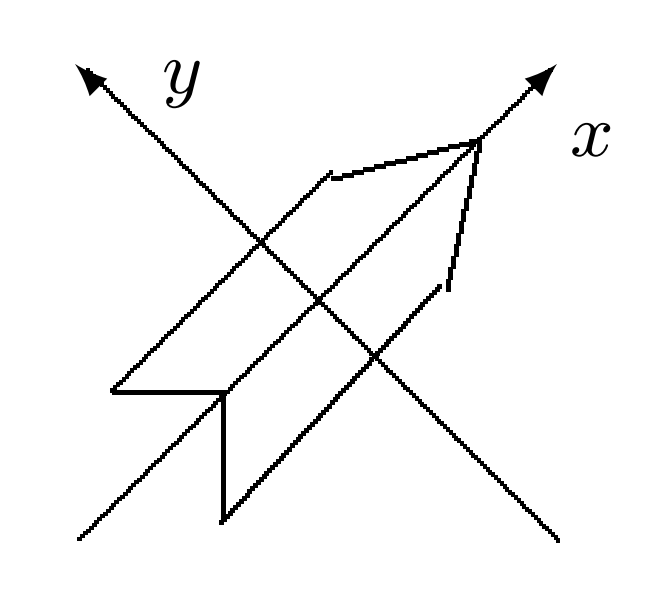
\includegraphics[width=0.2\linewidth]{pics/pic_3.png}
	\caption{{Пластинка чувствительного оттенка}}
	\label{pic_3}
\end{figure}

Выше предполагалось известным, какому из двух главных направлений пластинки в четверть длины волны соответствует большая скорость распространения света.
Установить это можно различными способами, например с помощью
пластинки чувствительного оттенка (так называют пластинку в $\lambda$
для зелёной спектральной компоненты, $\lambda = 560$ нм).

Пластинка имеет форму стрелы (рис. 3), вдоль оси которой расположено главное направление, соответствующее большей скорости распространения.

Если пластинка чувствительного оттенка помещена между скрещенными поляроидами и главные направления пластинки не параллельны
направлениям разрешённых колебаний поляроидов, то при освещении
белым светом пластинка кажется окрашенной в лилово-красный цвет.
Это объясняется тем, что зелёная компонента линейно поляризованного света при прохождении пластинки не меняет поляризации и задерживается вторым поляроидом. Для красной и фиолетовой компонент
пластинка создаёт сдвиг фаз, несколько отличный от $ 2\pi $. На выходе
из пластинки красная и фиолетовая компоненты оказываются поэтому
эллиптически поляризованными и частично проходят через второй поляроид. Таким образом, в известном смысле наблюдаемый в указанном
опыте цвет пластинки дополнителен к зелёному.

Если между скрещенными поляроидами поместить пластинку чувствительного оттенка
($ \lambda $) и пластинку в $ \lambda/4 $ так, чтобы их главные
направления совпадали, цвет пластинки изменится. Если у пластинки чувствительного оттенка и пластинки в $ \lambda/4  $совпадут главные направления, соответствующие большей скорости распространения, то разность хода между $ E_x $ и $ E_y $ для зелёного света составит уже $ 5\lambda/4 $. Это соответствует разности хода в $ \lambda $ для света с большей длиной волны, т. е. для "<более красного"> света. При освещении
этих пластинок (напомним, что они расположены между скрещенными поляроидами) белым светом теперь погасится не зелёная, а красная
часть спектра, и проходящий свет будет казаться зеленовато-голубым.
Если же главные направления, соответствующие большей скорости распространения, у пластинки чувствительного оттенка и у пластинки
в $ \lambda/4 $ окажутся перпендикулярными, то проходящий свет приобретёт
оранжево-желтую окраску (погасится фиолетово-голубая часть спектра).

Изменение цвета позволяет, таким образом, определить, какое из
главных направлений пластинки в $ \lambda/4 $ соответствует большей скорости
распространения.

\subsubsection{Интерференция поляризованных лучей}

\begin{figure}[!hb]
	\centering
	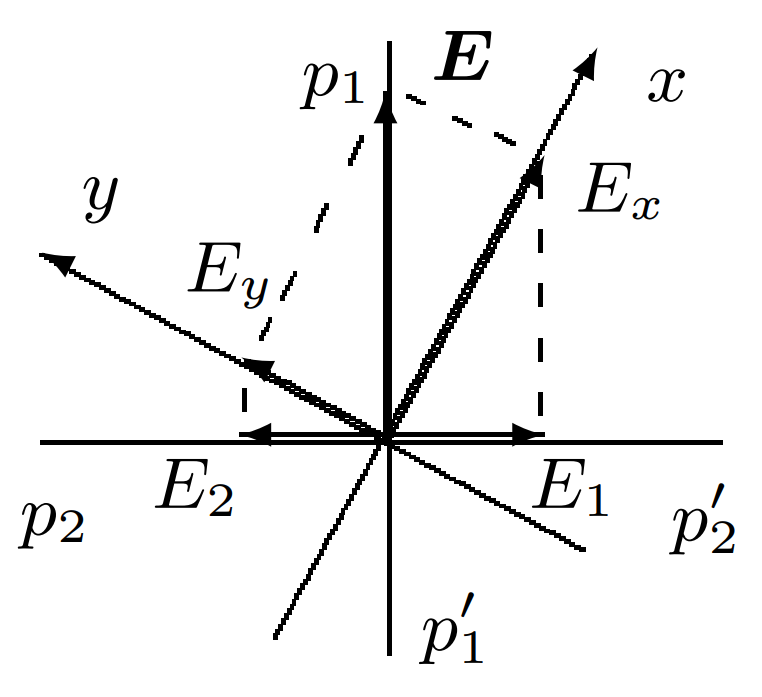
\includegraphics[width=0.25\linewidth]{pics/pic_4.png}
	\caption{{К объяснению интерференции поляризованных лучей}}
	\label{pic_4}
\end{figure}

Тонкие двоякопреломляющие пластинки, помещённые между поляроидами, кажутся окрашенными. Эта окраска может быть истолкована как результат интерференции поляризованных лучей. На рис. 4 представлена схема для
случая скрещенных поляроидов.

Здесь $ p_1p'_1 $ --- разрешённое направление колебаний поляризатора
(первого поляроида); $ x, y $ --- координатная система, связанная с главны-
ми направлениями двоякопреломляющей пластинки; $ p_2p'_2 $ --- разрешённое направление колебаний анализатора (второго поляроида). Волны
$ E_x  $ и $ E_y $ на выходе из пластинки когерентны, но не могут интерферировать, так как $ E_x \perp  E_y $. Волны $ E_1 $ и $ E_2 $ на выходе второго поляроида
также являются когерентными и к тому же поляризованы в одной плоскости. Эти волны интерферируют между собой. Результат интерференции определяется зависящим от длины волны сдвигом фаз между $ E_1 $
и $ E_2 $. В результате интерференции поляризованных лучей пластинка, освещаемая белым светом, кажется окрашенной.

Если поворачивать двоякопреломляющую пластинку, расположенную между
скрещенными поляроидами, то соотношение амплитуд волн $ E_1 $ и $ E_2 $ и разность фаз между ними не изменяются. Это означает, что цвет пластинки при её поворотах не меняется, а меняется только интенсивность света. За один оборот пластинки интенсивность четыре раза обращается в нуль --- это происходит при совпадении главных направлений
$ x $ и $ y $ с разрешёнными направлениями колебаний поляроидов.

Если же двоякопреломляющую пластинку оставить неподвижной, а
второй поляроид повернуть так, чтобы разрешённые направления $ p_1p'_1 $
и $ p_2p'_2 $ совпали, то волны $ E_1 $ и $ E_2 $ приобретают дополнительный фазовый сдвиг на $ \pi $ для всех спектральных компонент; при этом их амплитуды изменятся так, что цвет пластинки изменится на дополнительный. 

%-------------------------------------------------
\newpage

%-------Prac---------------------------
\subsection{Ход работы, результаты}
\paragraph{Первая часть работы} Для дальнейшей работы с поляризованным светом мы собрали следующую схему: Источник (далее И) -- Поляризатор (далее $P_1$) -- Черное зеркало (далее ЧЗ).

Вращая поляроид вокруг оси системы и зеркало в перпендикулярной оси, получили минимальную яркость пучка. В этот момент выполняются два условия:
\begin{enumerate}
    \item Свет падает на зеркало под углом Брюстера. Этот угол составил $\varphi_\text{Б} = 54^\circ$.
    \item На зеркало падает поляризованный свет, вектор $\textbf{E}$ параллелен плоскости падения. Таким образом, найдено горизонтальное положение разрешенной плоскости поляризатора $P_1$.
\end{enumerate}

\paragraph{Вторая часть работы} -- определение показателя преломления эбонита через угол Брюстера.

Чтобы найти угол Брюстера эбонитовой пластинки, мы установили ее вместо черного зеркала в прошлую установку. Полученная схема: <<И -- $P_1$ -- Э>>. Далее аналогично предыдущему пункту, получена минимальная интенсивность прошедшего пучка. По значению угла Брюстера по формуле \eqref{BrewstersAngle} определён показатель преломления эбонита. Экспериментальные данные:

\begin{table}[!ht]
    \centering
    \begin{tabular}{|l|l|l|}
    \hline
        Угол Брюстера эбонита & Угол поворота \varphi_\text{Б}, $^{\circ}$ & Показатель преломления $n$ \\ \hline
        Белый свет, мин & 49,5$\pm$1 & 1,17$\pm$0,02 \\ \hline
        Белый свет, макс & 53$\pm$1 & 1,32$\pm$0,02\\ \hline
        Белый свет среднее & 51$\pm$2 & 1,23$\pm$0,04 \\ \hline
        Зеленый свет среднее & 54$\pm$2 & 1,38$\pm$0,04 \\ \hline
    \end{tabular}
\end{table}

Табличное значение показателя преломления эбонита: $n_\text{табл} = 1,6-1,7$. Отклонение экспериментального значения от табличного довольно значительно~-- приблизительно $15-25\%$.

\paragraph{Третья часть работы} -- исследование стопы стеклянных пластинок.
При прохождении через стопу стеклянных пластинок отраженный и преломленный свет поляризуется. Для исследования явления мы установили зеленый фильтр на источник, выделив часть спектра. После фильтра свет пропускается через стопу, а преломленный и отраженный пучки исследуются при помощи поляризатора $P_1$. Схема установки изображена на рис. \ref{Stopa}. 

\begin{figure}[!hb]
	\centering
	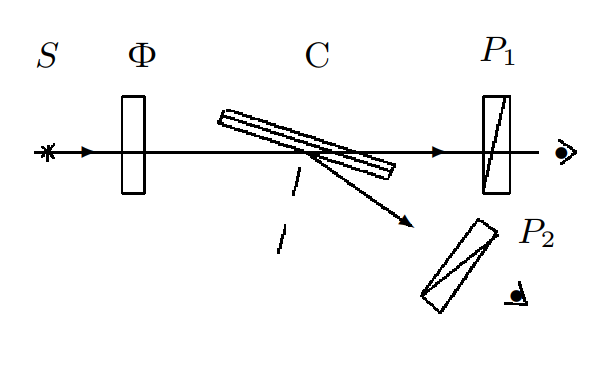
\includegraphics[width=0.5\linewidth]{pics/Stopa.png}
	\caption{{Исследование стопы пластинок}}
	\label{Stopa}
\end{figure}

Интенсивность отраженного пучка минимальна, когда поляризатор установлен горизонтально. Для преломленного луча напротив -- положение поляризатора, отвечающее минимальной интенсивности пучка, вертикально. 

Так как минимальность интенсивности достигается при перпендикулярности разрешенной плоскости поляризатора и плоскости поляризованного пучка, можно сделать следующие выводы:
\begin{enumerate}
    \item Отраженный пучок получает <<вертикальную>> поляризацию, то есть перпендикулярную плоскости падения луча.
    \item Преломленный пучок напротив, имеет <<горизонтальную>> поляризацию, то есть параллельную плоскости падения.
\end{enumerate}

\paragraph{Четвертая часть работы} -- определение толщины двоякопреломляющих пластинок. 

Согласно теоретическому введению, линейно поляризованный монохроматический свет, проходя через пластинку с толщиной $\frac \lambda 2$, меняет положение вектора поляризации на зеркальное относительно главной оси пластинки. При этом результирующий пучок остается линейно поляризованным. В случае, когда толщина пластинки составляет $\frac \lambda 4$, прошедший пучок имеет круговую поляризацию. 

В экспериментальной установке, изображенной на рис. \ref{lambda}, поляризаторы $P_1$ и $P_2$ были установлены таким образом, чтобы выходящий пучок был минимальной интенсивности, то есть их разрешенные плоскости скрещены. 

Вращая пластинки вокруг пучка, мы добились минимальной интенсивности исходящего луча. Для двух пластинок наблюдались различные результаты:
\begin{enumerate}
    \item Для первой пластинки на выходе интенсивность была практически нулевая. Это означает, что выходящий пучок линейно поляризован и имеет плоскость поляризации, перпендикулярную разрешенной плоскости $P_2$. Таким образом, можно сделать вывод о том, что эта пластинка имеет толщину $\frac \lambda 2$.
    \item Для второй пластинки на выходе интенсивность упала по сравнению с изначальной, однако не до нуля. Это означает, что выходящий пучок имеет круговую поляризацию, не имеющую выделенного направления. Следовательно, $P_2$ пропускает только половину светового пучка (если усреднить по времени), затемняя результат. Следовательно, эта пластинка имеет толщину $\frac \lambda 4$.
\end{enumerate}

\begin{figure}[!hb]
	\centering
	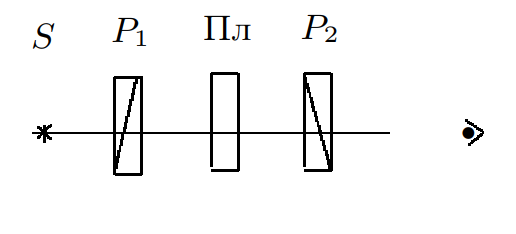
\includegraphics[width=0.5\linewidth]{pics/lambda.png}
	\caption{{Исследование двоякопреломляющих пластинок}}
	\label{lambda}
\end{figure}


\paragraph{Пятая часть работы} -- определение главных <<быстрой>> и <<медленной>> осей пластинки $\frac \lambda 4$.

Установив фильтр на источник, мы исследовали только зеленый свет с длиной волны примерно $\lambda = 550\text{нм}$. Далее между скрещенными поляроидами устанавливается пластинка $\lambda$. Положение $P_2$, максимально ослабляющее выходящий пучок не зависит от наличия пластинки, следовательно, она не меняет поляризацию зеленого пучка -- это подтверждает равенство ее толщины $\lambda$.

Далее мы убрали фильтр. Полученный пучок имеет пурпурно-красный цвет, что означает ослабление зеленого пучка при прохождении через систему. Этот эффект возникает из-за того, что поляризаторы $P_1, P_2$ не пропускают зеленый свет, не меняющий своей поляризации при прохождении через пластинку. Остальные же цвета изменяют угол от нее и ослабляются в меньшей степени поляризатором $P_2$.

Затем в систему была добавлена пластинка $\frac \lambda 4$. Полученная схема изображена на рис. \ref{fig:Axis}. При этом оси пластинки совпадают с главными остями пластинки $\lambda$, и ориентированы под углом $45^{\circ}$ к разрешённым направлениям скрещенных поляроидов. При повороте рейтера со стрелкой на $180^{\circ}$ вокруг вертикальной оси цвет стрелки меняется от зелёно-голубого до оранжево-жёлтого. При совпадении главных осей пластинок $\lambda$ и $\frac \lambda 4$ разность хода для зеленого пучка будет уже $\frac {5 \lambda} 4$, он выйдет из $P_2$. А вот для <<более красного>> света разность как раз станет составлять $\lambda_к$, и $P_2$ его задержит. Таким образом, в том случае, когда зеленый свет наиболее ярко виден после $P_2$, у пластинок совпадают оси.

\begin{figure}[!ht]
	\centering
	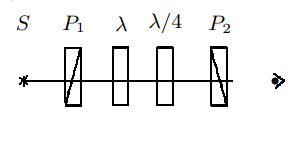
\includegraphics[width=0.5\linewidth]{pics/Axis.png}
	\caption{Определение направлений большей и меньшей скорости}
	\label{fig:Axis}
\end{figure}

\paragraph{Шестая часть работы} -- интерференция поляризованных лучей. 

Установка прошлого пункта модифицирована: вместо пластинки $\lambda$ выставлена  мозаичная слюдяная пластинка. Она собрана из 4-х узких полосок слюды, лежащих по сторонам квадрата (две полоски «толщиной» $\frac lambda 4$ и по одной — $\frac \lambda 2$ и $\frac{3\lambda}{4}$). В центральном квадратике слюды нет. Главные направления всех пластинок ориентированы параллельно сторонам квадрата.

При вращении поляроида угловые квадраты обесцвечиваются, а те, что вокруг (центра) - окрашиваются. Если вращать саму пластинку, изменяется интенсивность света. Оба процесса происходят с периодом в $\frac \pi 4$. Количественные результаты:

\begin{table}[!ht]
    \centering
    \begin{tabular}{|l|l|l|}
    \hline
        $3 \lambda / 4$ зеленый & $\lambda / 2$ пурпурный & $3 \lambda / 4$ зелёный \\ \hline
        $\lambda / 4$ красный   & -                       & $\lambda / 4$ красный \\  \hline
        $\lambda $ желтый       & $3 \lambda / 4$ синий   & $\lambd $ желтый \\ \hline
    \end{tabular}
\end{table}

\paragraph{Седьмая часть работы} -- определение направления вращения вектора в эллиптически поляризованном свете.

\begin{figure}[!ht]
	\centering
	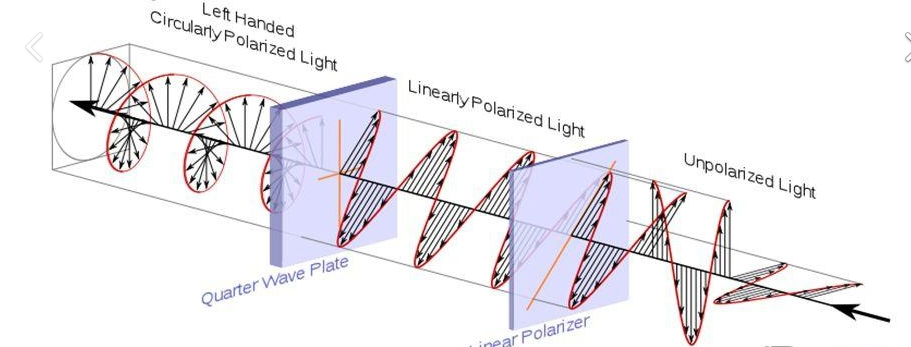
\includegraphics[width=0.5\linewidth]{pics/3D.png}
	\caption{Эллиптическая поляризация}
	\label{fig:3d}
\end{figure}

\begin{figure}[!ht]
	\centering
	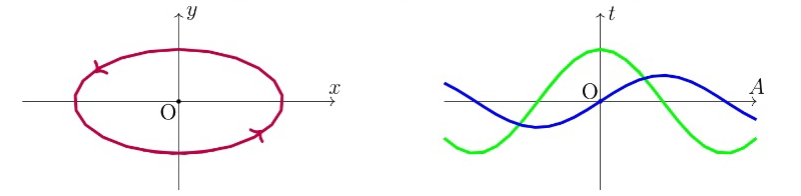
\includegraphics[width=0.5\linewidth]{pics/ellipses.png}
	\caption{Графики синусов}%лол
	\label{fig:ellipses}
\end{figure}

Из графиков, представляющих собой фазы света, распространяющегося вдоль разных осей, видно, что вращение вектора будет осуществляться против часовой стрелки, если смотреть против пучка.

%-------Results---------------------------
\subsection{Выводы}
В данной работе было изучено явление поляризации света при прохождении через поляроиды и двояко двоякопреломяющие пластинки. Определен угол Брюстера для эбонита, который составил приблизительно $51^\circ$. 

Основное исследование посвящено созданию двоякопреломяющими пластинками разности хода между ортогональными компонентами световой электромагнитной волны. Данный эффект приводит к изменению положения вектора поляризации или возникновению явления эллиптической поляризации, в зависимости от соотношения длины волны и толщины пластинок. 

При помощи набора пластинок с различной толщиной ($\lambda, \lambda / 2, \lambda / 4$ можно получить эллиптическую поляризацию, причем установлено, что вектор напряженности будет вращаться против часовой стрелки. Толщину пластинки можно определять при помощи скрещенных поляроидов и цветового фильтра, воспользовавшись зависимостью вышеперечисленных явлений от длины волны.